

The MusEEG root directory (Figure~\ref{fig:projectStructure})  consists of a data directory, an example scripts directory, the MusEEG library, a README file, a library requirements file, a demo application, and an MIT License file.

 \begin{figure}[H]
	\centering
		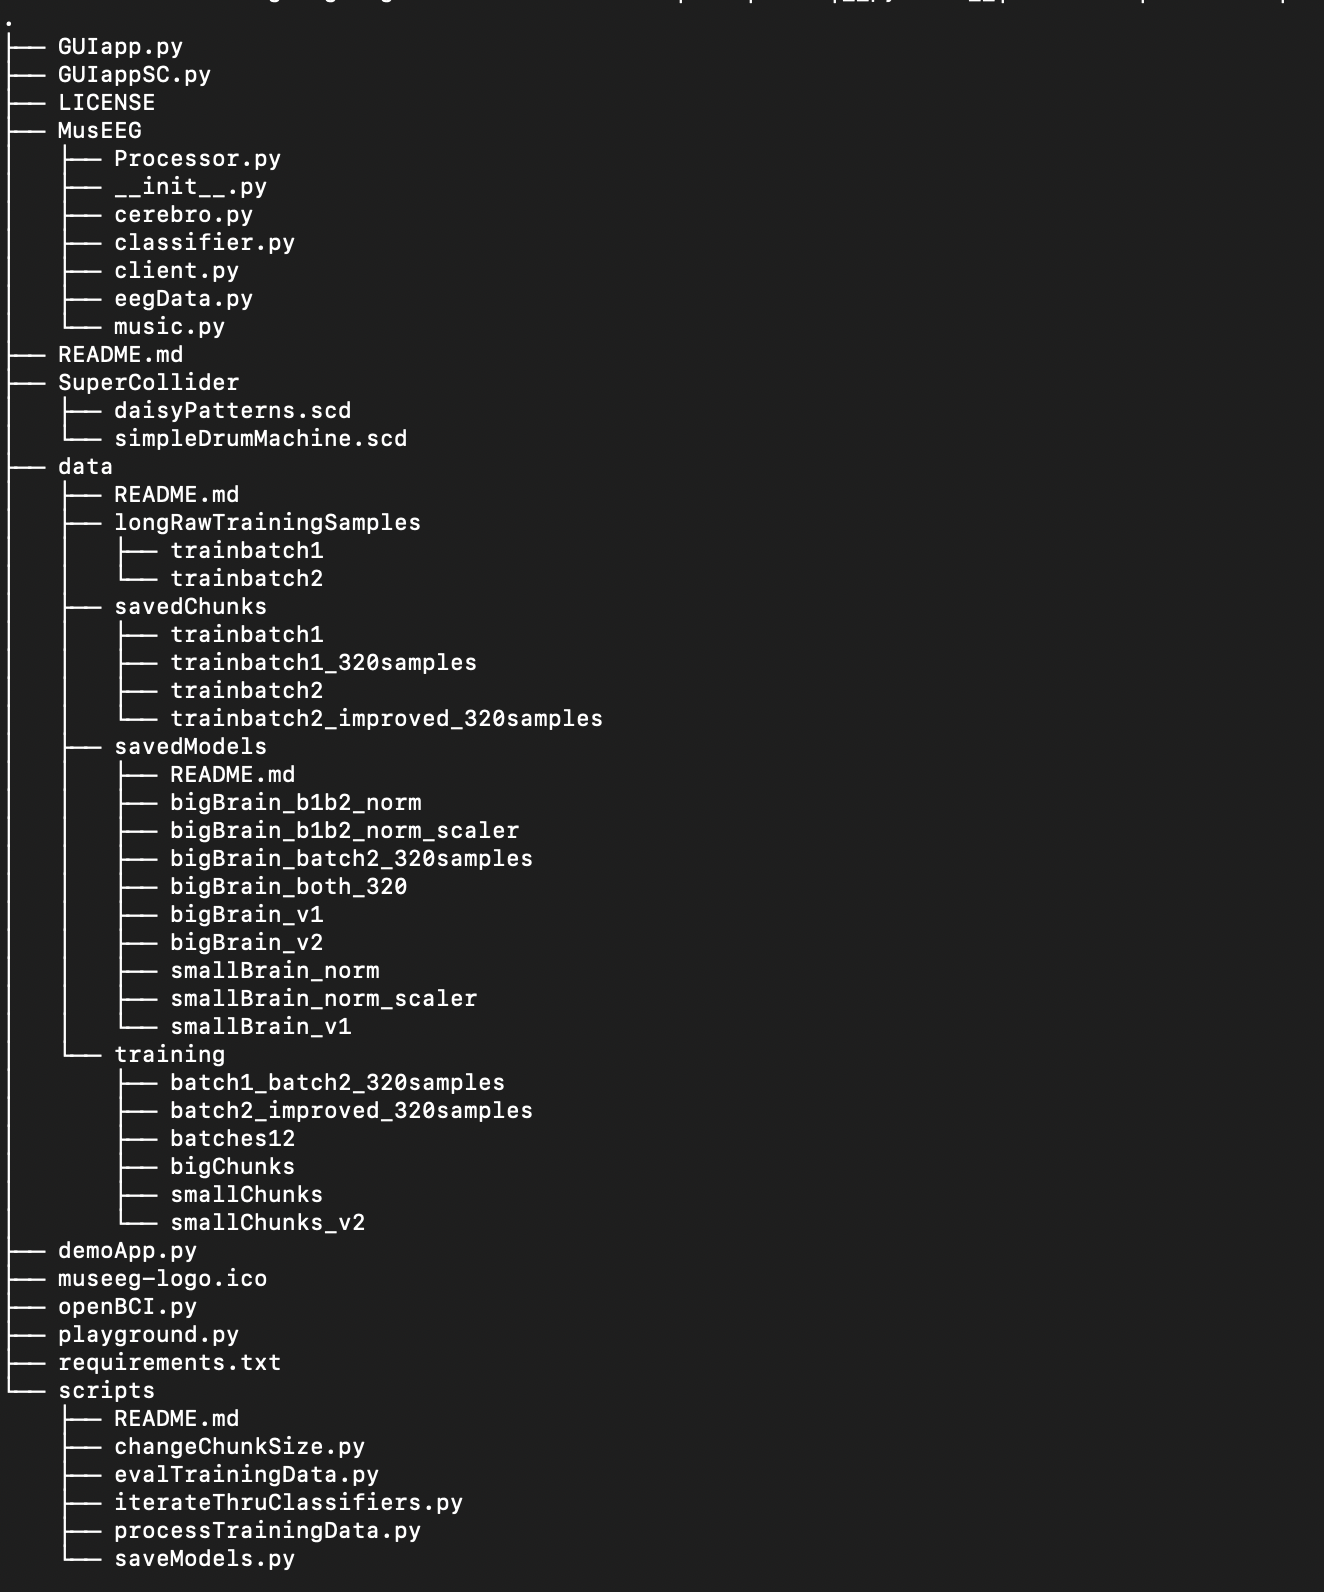
\includegraphics[width=0.8\columnwidth]{projectStructure.png}
	\caption{MusEEG Project Structure}
	\label{fig:projectStructure}
\end{figure} 

\pagebreak

\section{The Data Directory}
The /data directory of the MusEEG module stores EEG data in all of its different training stages, inputs and targets for the ANN models, as well as the ANN models themselves. The /data/longRawTrainingSamples subdirectory stores .csv files with multiple samples of a single gesture. During the normal workflow of the data acquisition process, the files from the longRawTrainingSamples subdirectory are curated and stored into individual chunks in the /data/savedChunks subdirectory, which in itself contains subdirectories for smallChunks and bigChunks. The /data/savedModels subdirectory saves Keras models that have been trained and are ready for usage, while the /data/training subdirectory stores preprocessed and prelabeled input and target vectors for designing ANN models.



\section{MusEEG Library}
The MusEEG library contains all the required classes to build a brain-computer interface for music performance. It is organized into five modules:
\begin{itemize}
\item eegData.py (import, process, plot, save EEG data).
\item music.py (MIDI objects, chords, and melodies)
\item classifier.py (build, train, save keras models easily)
\item cerebro.py (methods to use music, classifier, and eegData together)
\item client.py (TCP client setup to receive live raw EEG data stream from EPOC+ headset and stream .csv giles)
\item Processor.py (real-time processing and OSC communication)
\end{itemize}

 \begin{figure}[H]
	\centering
		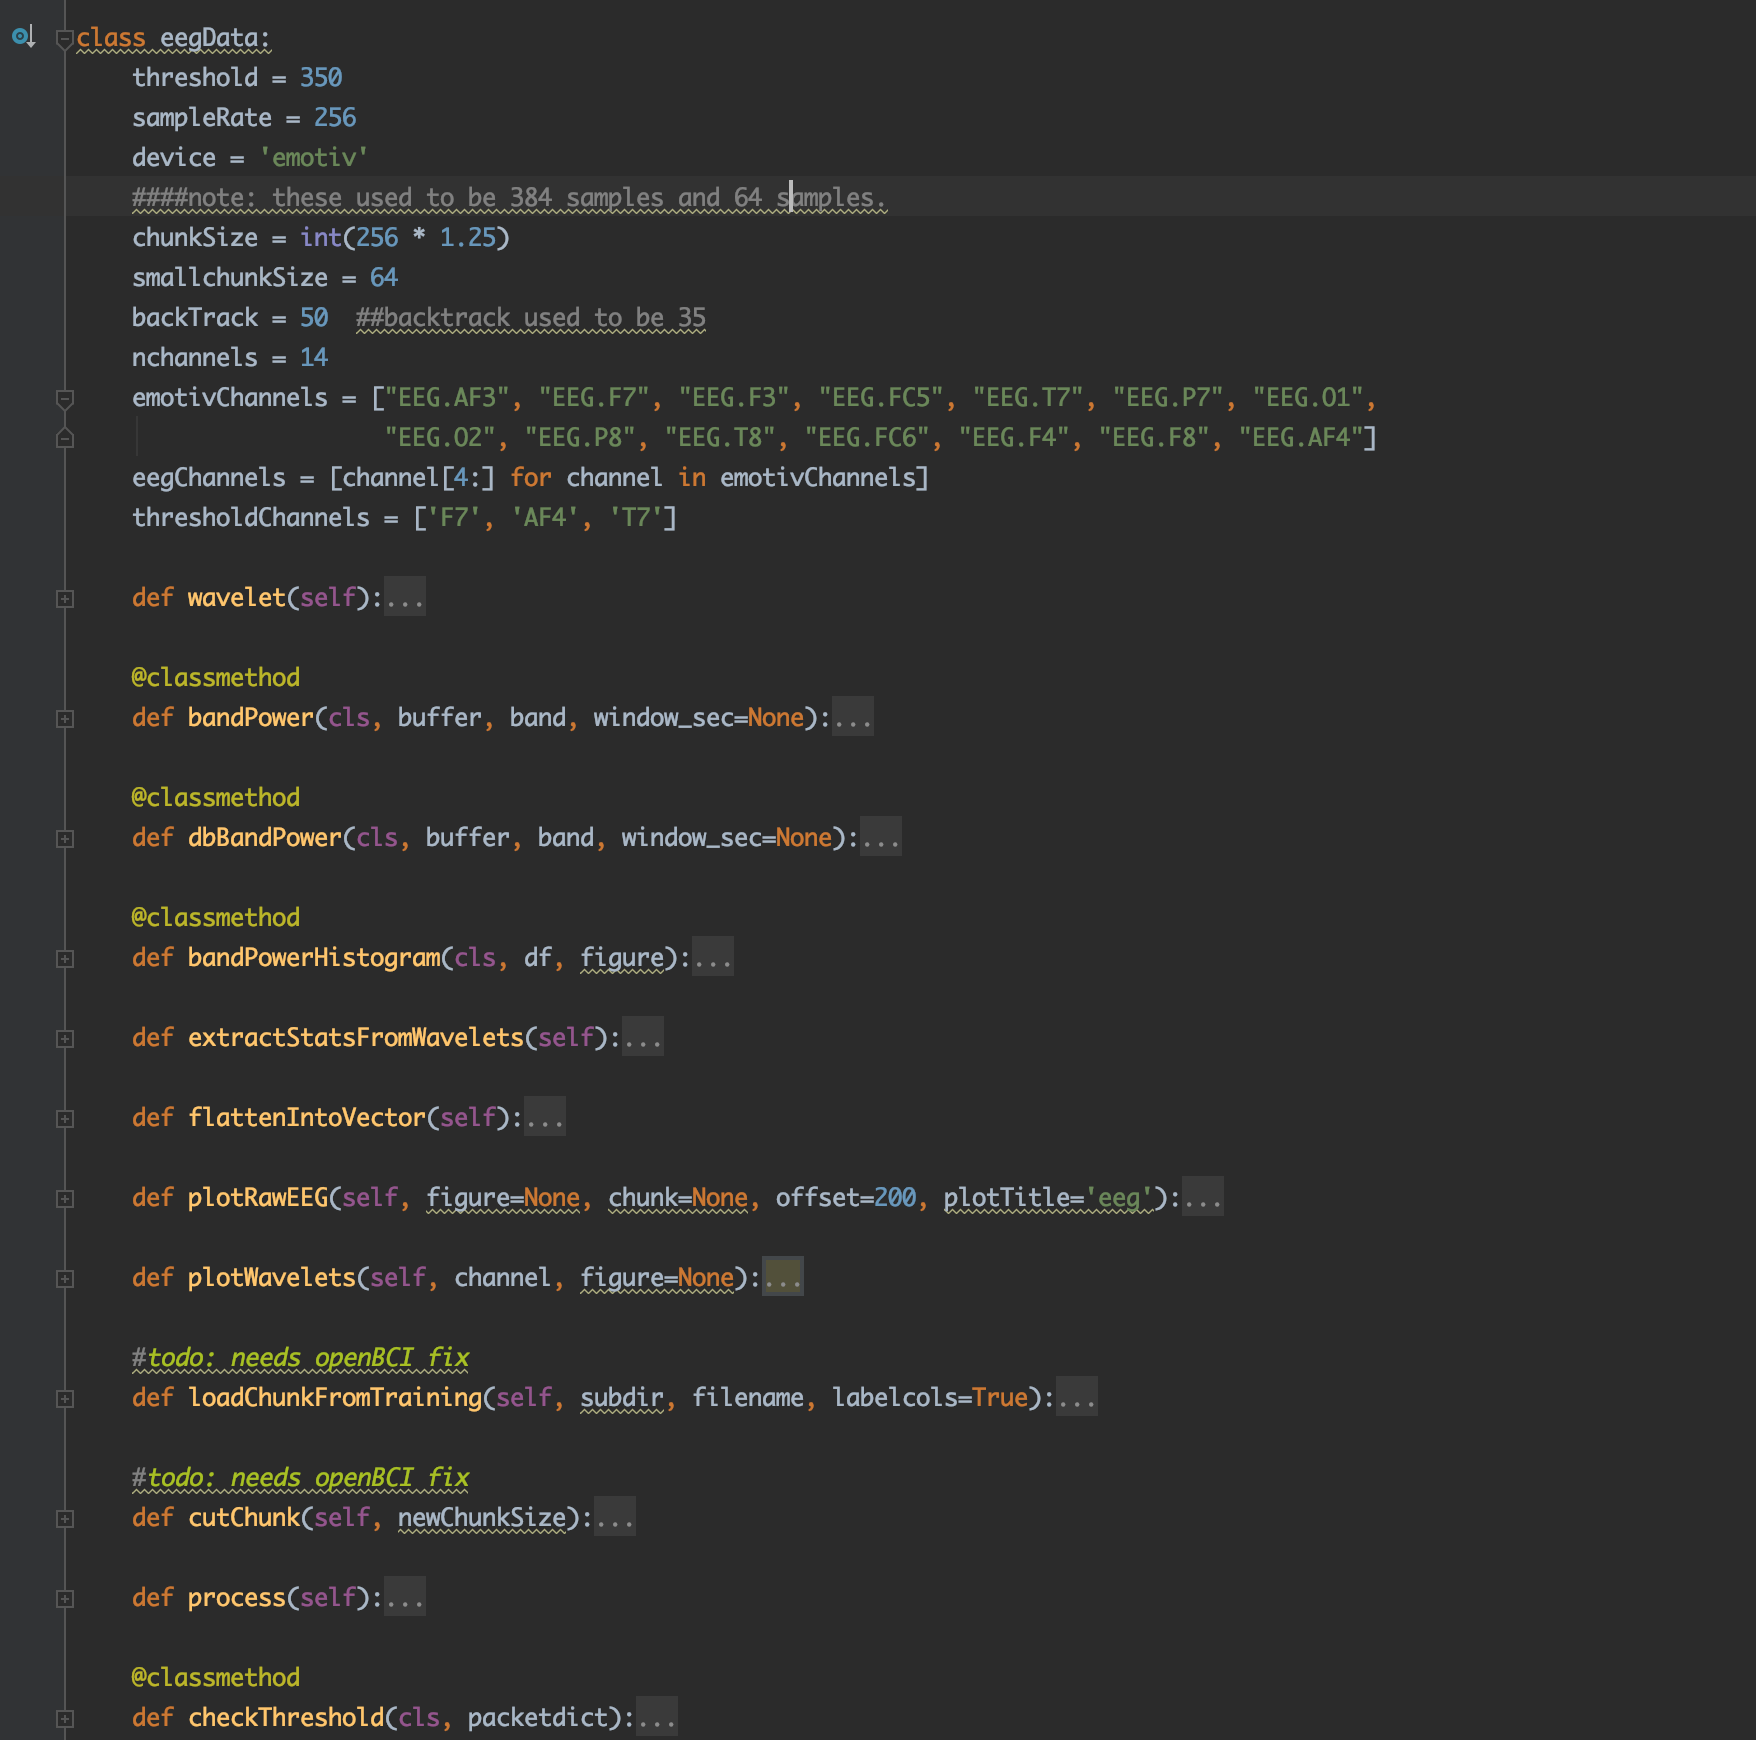
\includegraphics[width=1\columnwidth]{eegDataClass.png}
	\caption{Overview of eegData class methods}
	\label{fig:eegDataClass}
\end{figure} 

\bigskip
The eegData class (Figure~\ref{fig:eegDataClass}) helps a user import raw EEG data from .csv files, curate it into processable chunks, process using wavelet decomposition and statistical extraction, as well as plot the 14-channel EEG signal or the five coefficient vectors created by the wavelet decomposition. It is currently designed around the EPOC+ model, but can be redesigned for any other EEG system, provided that the developer has a means of obtaining a raw EEG stream from such system. The eegData class builds upon the PyWavelets, matplotlib, SciPy, and Pandas Python libraries. 

\begin{figure}[H]
	\centering
		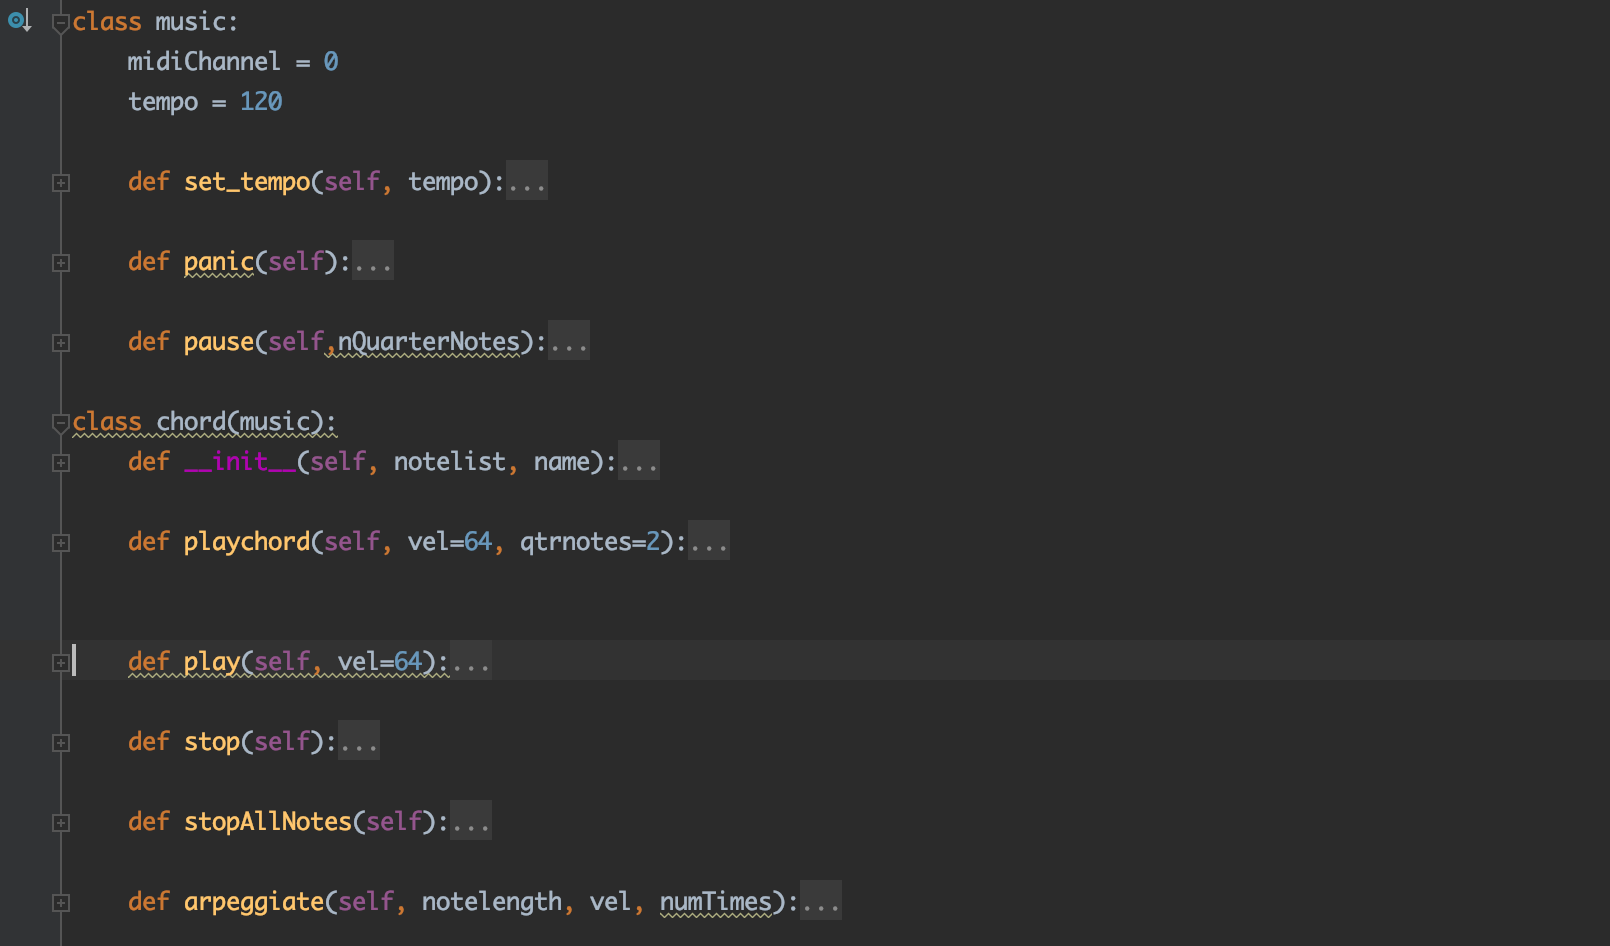
\includegraphics[width=1\columnwidth]{musicClass.png}
	\caption{Overview of music class methods}
	\label{fig:musicClass}
\end{figure} 

	The music class (Figure~\ref{fig:musicClass}) is designed to allow the user to create, load, and save different MIDI events for use during performance. As of now, the music class allows the creation of chord and melody objects, though future iterations will also include the option to load pre-written MIDI files created using third-party MIDI sequencing software. The music class is built upon the Mido and Audiolazy libraries. 

\begin{figure}[H]
	\centering
		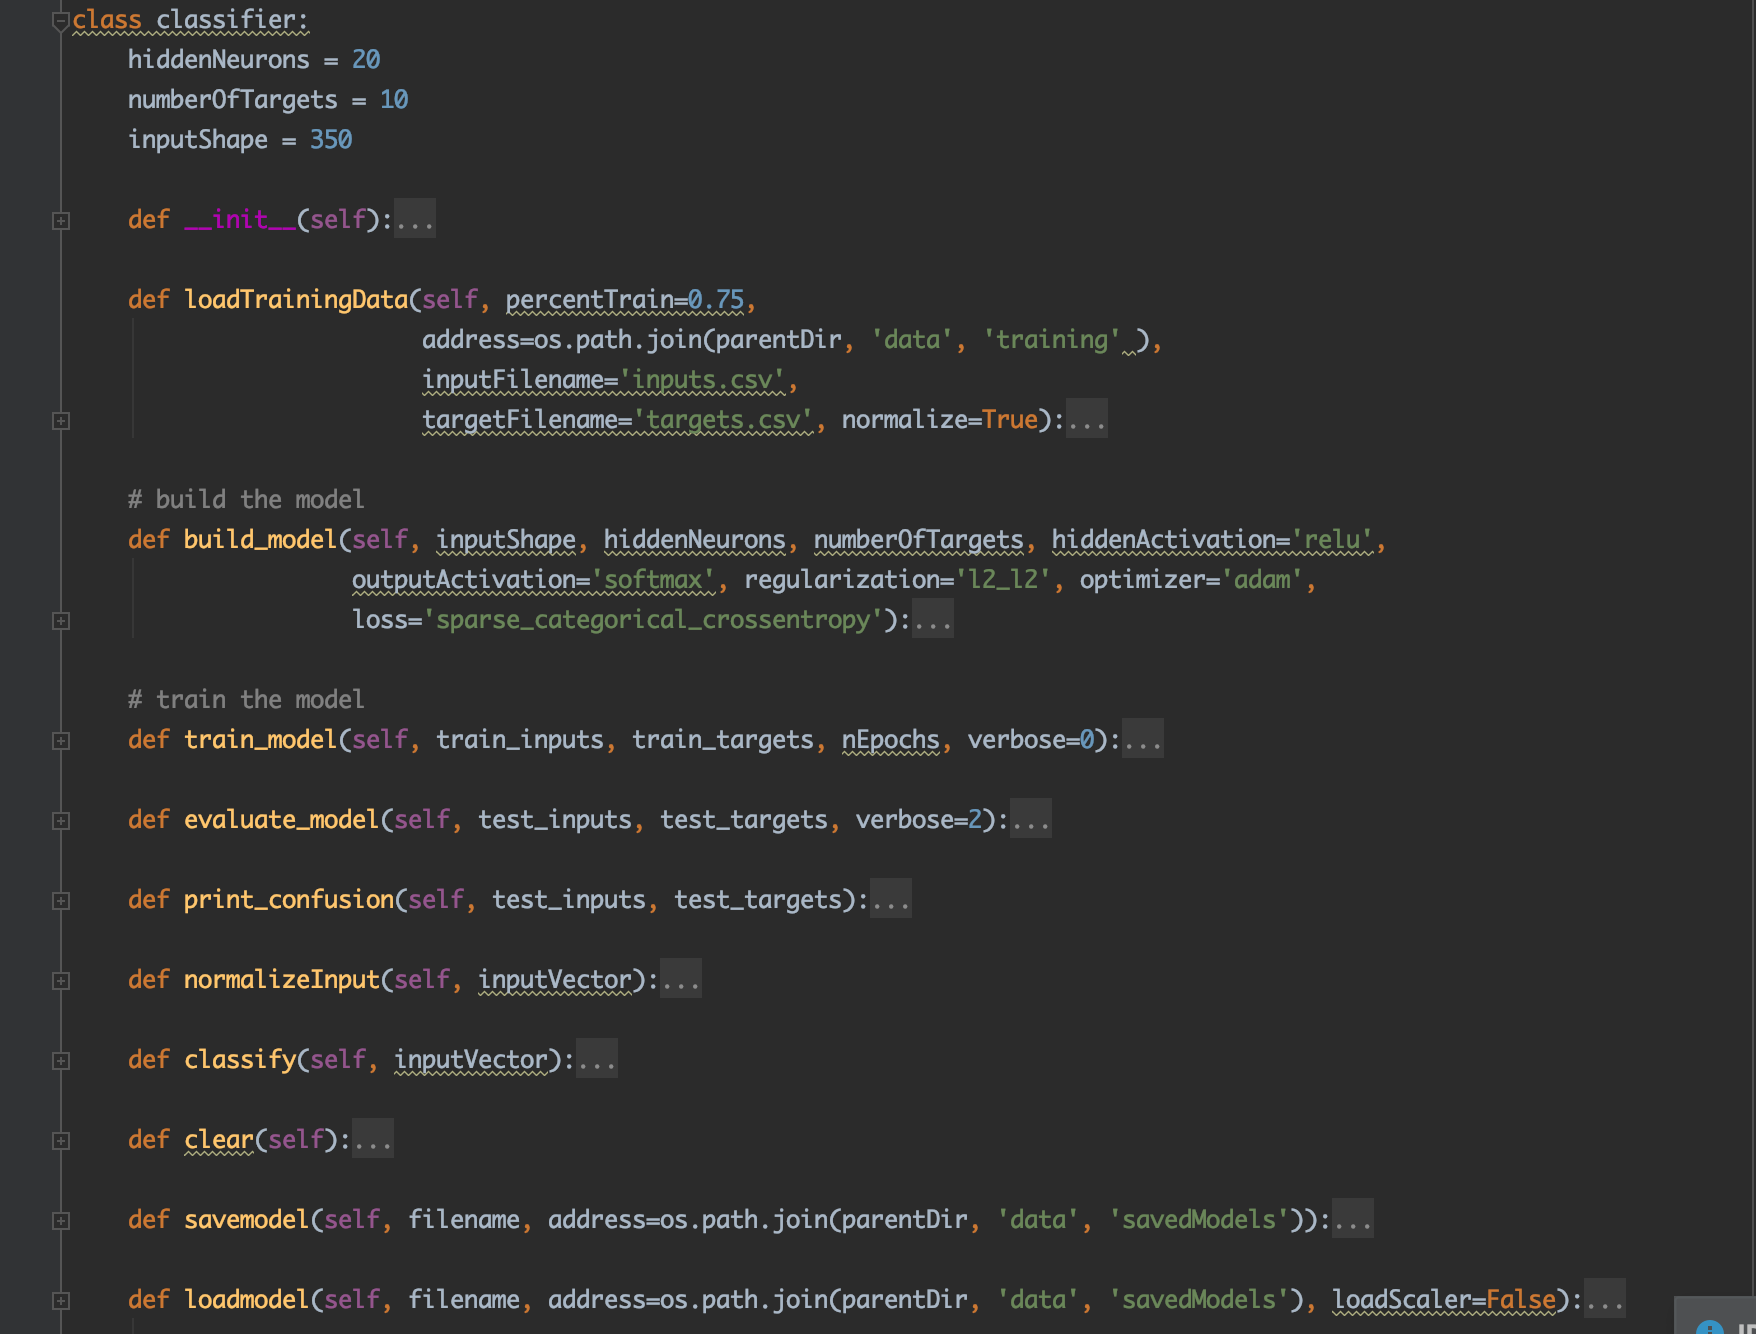
\includegraphics[width=1\columnwidth]{classifierClass.png}
	\caption{Overview of classifier class methods}
	\label{fig:classifierClass}
\end{figure} 
 
	The classifier class (Figure~\ref{fig:classifierClass}) builds upon the TensorFlow and Keras libraries to expedite the process of creating, training, loading, saving, and analyzing the performance of ANN models. 

\begin{figure}[H]
	\centering
		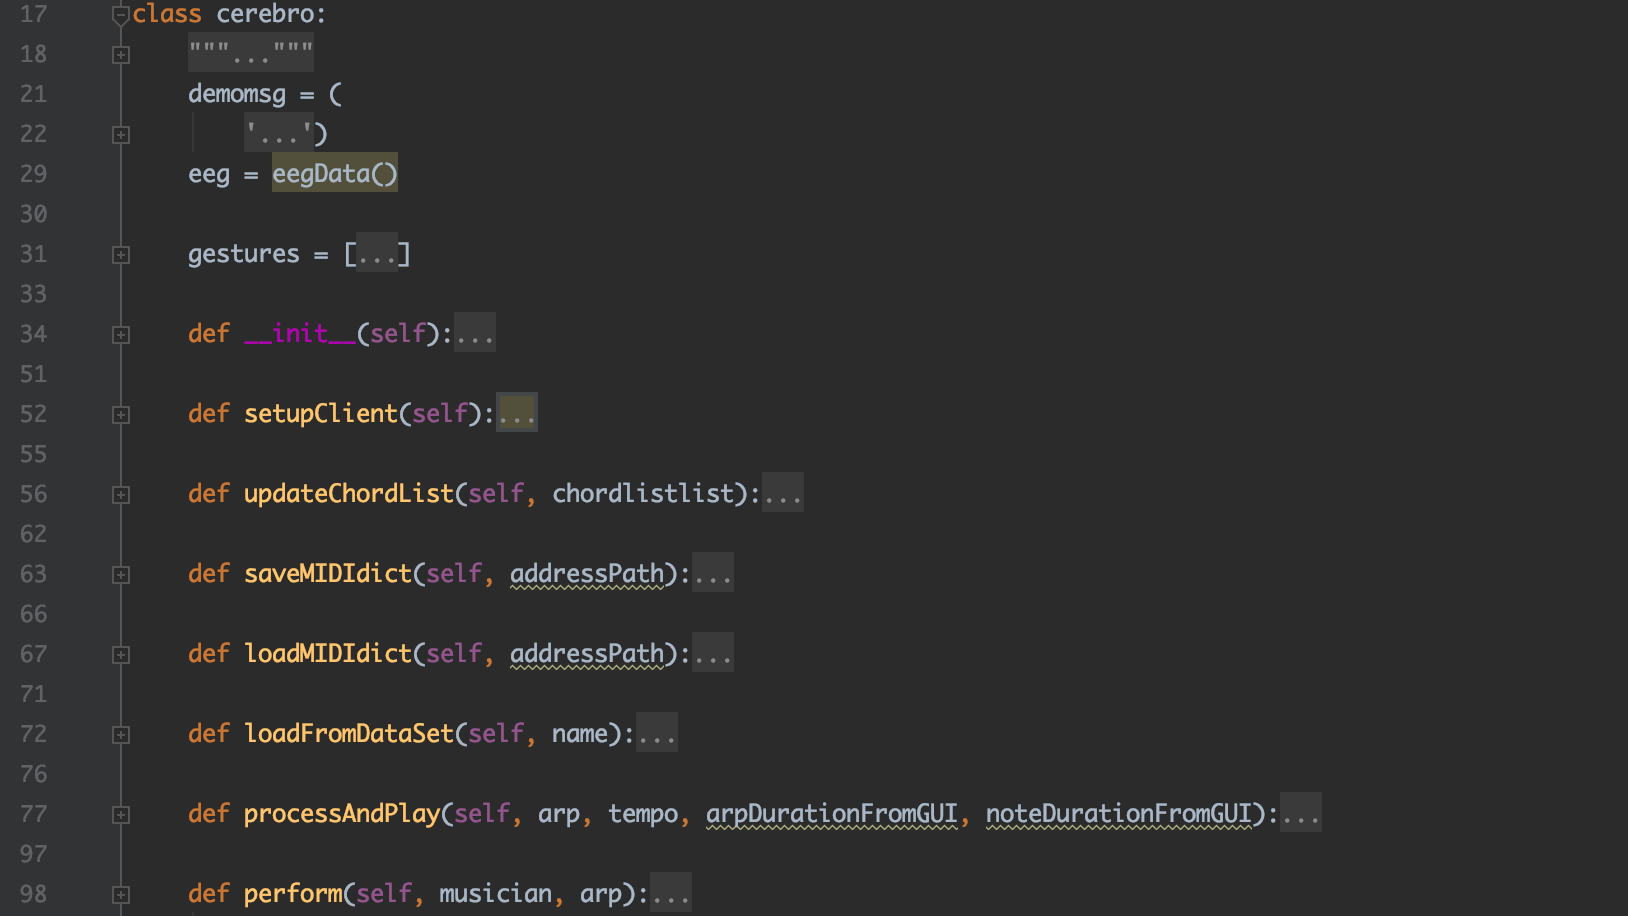
\includegraphics[width=1\columnwidth]{cerebroClass.png}
	\caption{Overview of cerebro class methods}
	\label{fig:cerebroClass}
\end{figure}  
 
	The cerebro class serves as a high-level API for less experienced programmers to make use of the MusEEG package, as it contains methods that use the eegData, classifier, and music classes in conjunction to create brain-computer music interface systems. The cerebro class is built on top of the eegData, music, classifier, and client classes from the MusEEG package.

\begin{figure}[H]
	\centering
		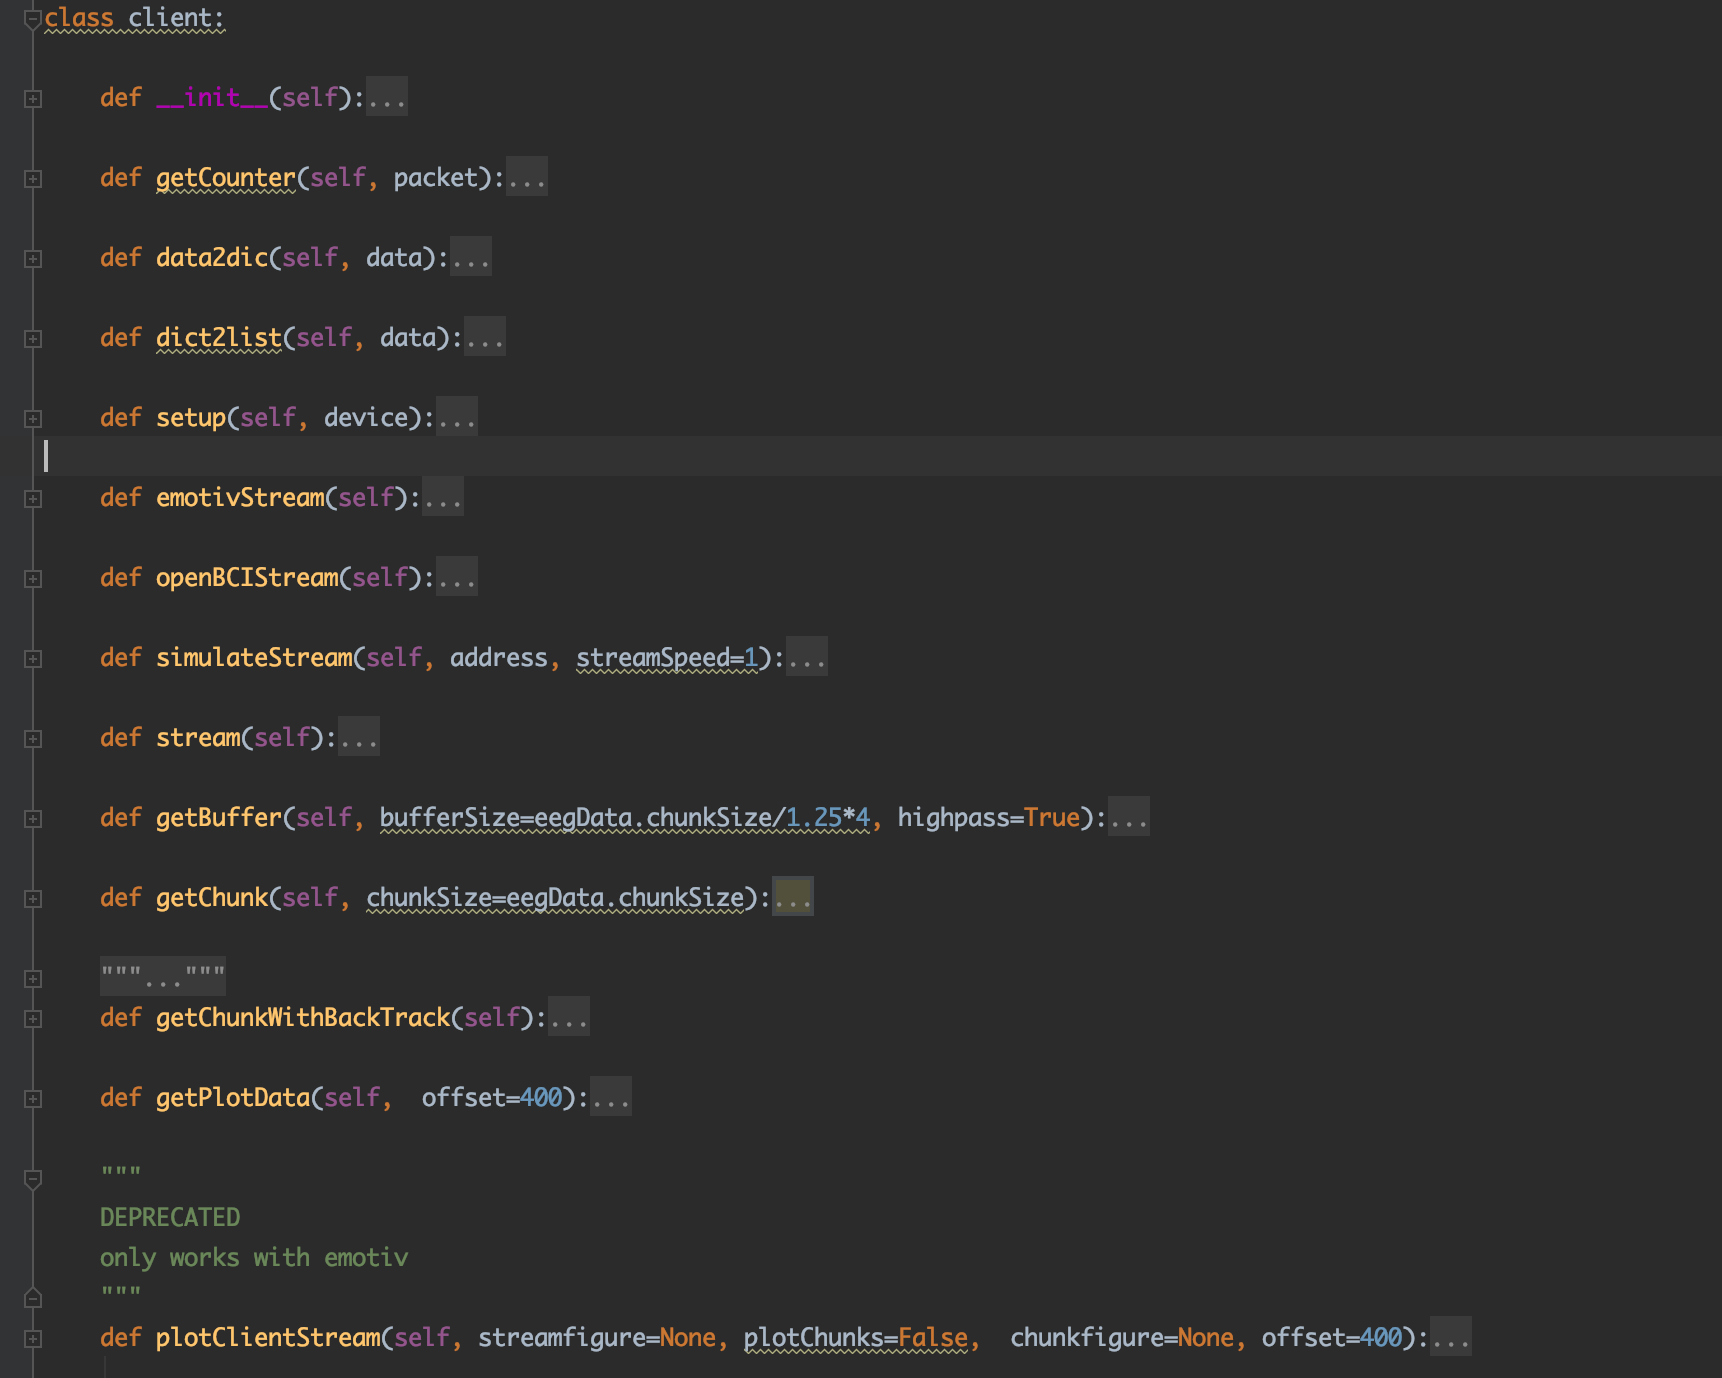
\includegraphics[width=1\columnwidth]{clientClass.png}
	\caption{Overview of client class methods}
	\label{fig:clientClass}
\end{figure}  
 

The client class (Figure~\ref{fig:clientClass}) sets up a TCP client that receives raw EEG data packets from an EEG stream server and packs them into chunks to create eegData objects. The client class is also capable of creating a raw EEG streaming simulation by effectively streaming a pre-recorded .csv EEG session into the server. 


\begin{figure}[H]
	\centering
		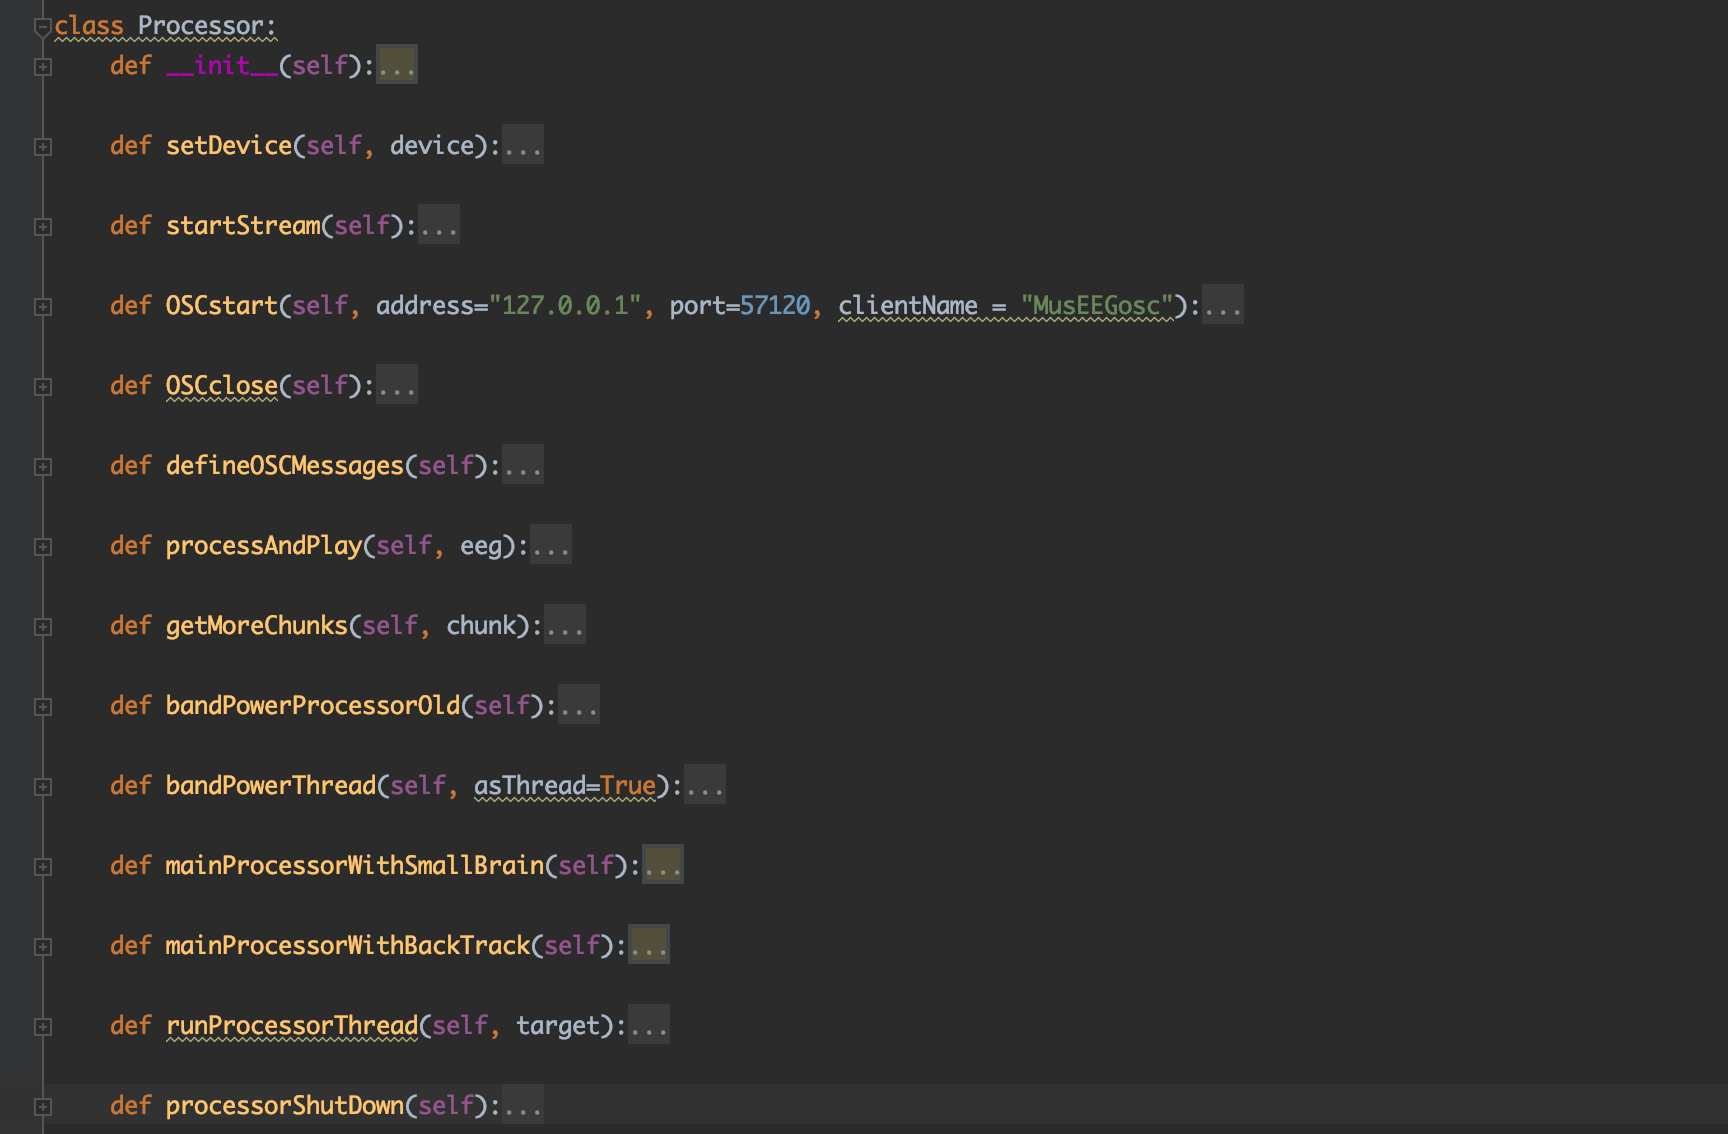
\includegraphics[width=1\columnwidth]{processorClass.png}
	\caption{Overview of Processor class methods}
	\label{fig:processorClass}
\end{figure}  
 

The processor class (Figure~\ref{fig:processorClass}) contains real-time processing methods that communicate with the client and eegData classes to perform real-time EEG classification and MIDI/OSC processing as described in (Figure~\ref{fig:realTimeFlowChart}) and (Figure~\ref{fig:processorwithwakeup}).

\pagebreak
\section{Example Scripts}

The MusEEG/scripts directory contains a series of sample scripts that can be useful during the creation of a user’s training samples and ANN model.

evalTrainingData.py provides an example of importing long .csv files that contain multiple samples of the same gesture from the MusEEG/data/longRawTrainingSamples directory and using the TrainingDataMacro class to evaluate, curate, and save individual training samples to the /data/savedChunks directory.

\begin{figure}[H]
	\centering
		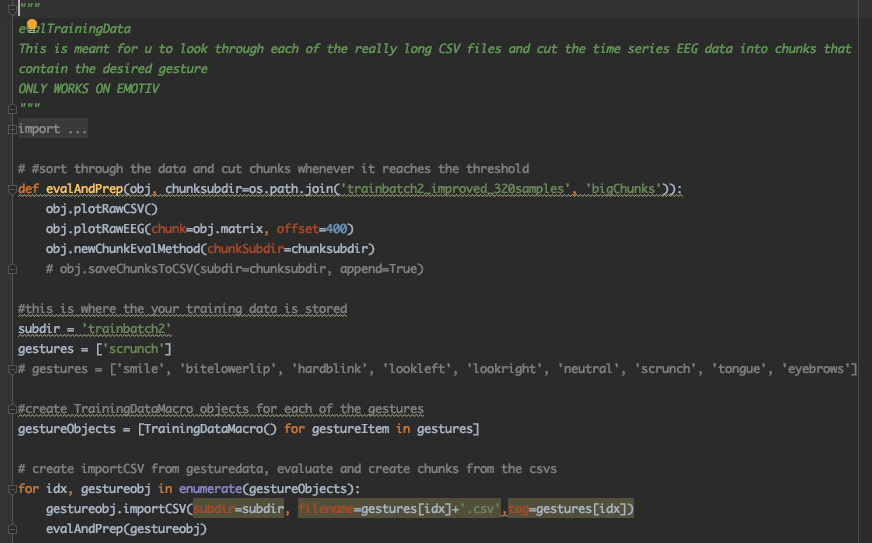
\includegraphics[width=1\columnwidth]{evalTrainingData.png}
	\caption{evalTrainingData Script}
	\label{fig:evalTrainingData}
\end{figure}  
 
\pagebreak
processTrainingData.py grabs the curated chunks from the /data/savedChunks directory and performs the preprocessing and feature extraction routine (wavelet transform and statistical extraction), as well as creates training inputs and targets and stores them in the /data/training directory.

\begin{figure}[H]
	\centering
		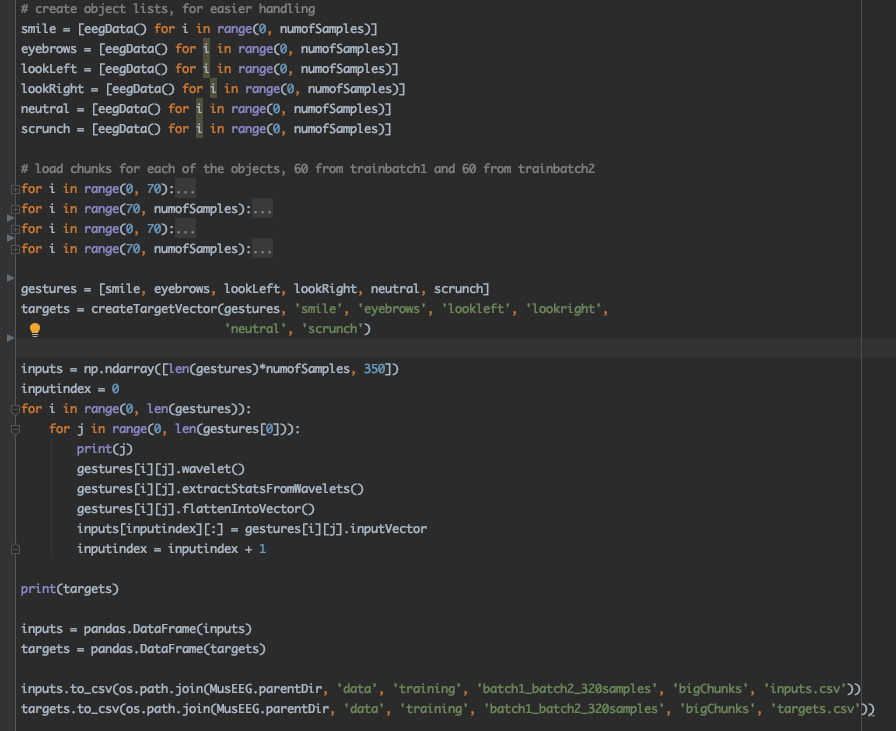
\includegraphics[width=1\columnwidth]{processTrainingData.png}
	\caption{processTrainingData Script}
	\label{fig:processTrainingData}
\end{figure}  
 \pagebreak

Because the dataset is quite small and one-dimensional, training ANN models is relatively computationally inexpensive. This lets a user perform an exhaustive search of different ANN models with different activation units, hidden layer sizes, and regularization parameters within the span of a couple of minutes. iterateThruClassifiers.py iterates over every combination of different hidden layer activation functions, output layer activations, regularization parameters, number of hidden neurons, and loss functions to find the one that performs with the highest accuracy. The iterateThruClassifiers.py script creates a .csv file in the /data/ClassifierOptimizations directory which contains the test results for each of the combinations tried. 
saveModels.py trains and saves a Keras model in the /data/savedModels directory.
